\documentclass{article}

\usepackage[margin=1.0in]{geometry}
\usepackage{graphicx}
\usepackage{amsmath}
\usepackage{float}

\title{CSC 535 HW1}
\date{8/30/2018}
\author{Simon Swenson}

\begin{document}

\pagenumbering{gobble}
\maketitle
\pagenumbering{arabic}

\large Introduction

\small I completed all required homework problems. For Q2, I went with method A 
(assuming no duplicate results) rather than method B.

\section{Q1}

As the number of dice throws (of 2d6) approach infinity, the experimental 
results should converge to the actual probability distribution. In this case, 
since we are checking two independent events (each die in the dice roll), we
\textit{could} create a chart for the possible outcomes. However, in this case, 
that is not really necessary. We know that a roll of 12 can only happen when 
each die comes up a 6. Therefore, we know the probability is $\frac{1}{n}$, 
where n is the number of possible outcomes (when both dice are considered). 
This is 36, since each die has six possible outcomes. Therefore, we expect the experimental 
results to converge to the value $\frac{1}{36} \approx 0.028 = 2.8 \%$. 
However, even after 1000 dice throws, the experimental results are off by a 
non-negligible amount. The first result of the random number generator was 
$3.3\%$, and only one of the ten experiments (each of 1000 throws) resulted in 
$3.3\%$ as well. However, reseeding the random number generator immediately 
yielded the same result, as expected:

\begin{enumerate}
    \item $3.3\%$
    \item $2.1\%$
    \item $2.9\%$
    \item $2.2\%$
    \item $2.6\%$
    \item $2.8\%$
    \item $2.5\%$
    \item $2.1\%$
    \item $3.3\%$
    \item $3.1\%$
    \item $3.3\%$ (after seed reset)
\end{enumerate}

In any large system that uses random number generation, the random seed is 
important for reproduceability and debugging. In the best-cased 
scenario, the initial state of the random number generator shouldn't 
matter, however, that's not always the case, especially when the system is 
still being built and debugged (from my experience with deep learning).

\section{Q2}

\begin{figure}[!ht]
	\centering
	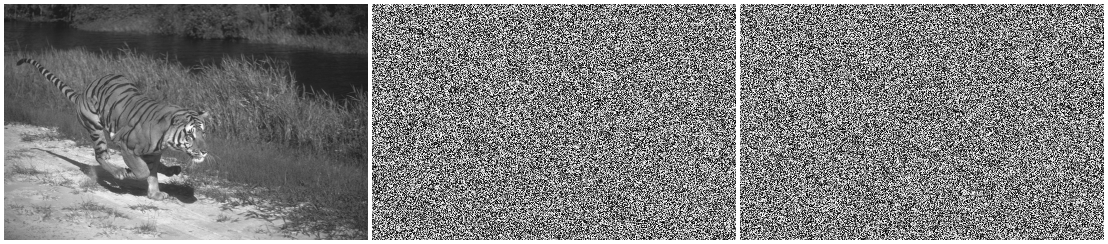
\includegraphics[width=180mm]{tiger-and-noise.png}
	\caption{So-called "Random noise," alongside two more pictures of random noise}
\end{figure}

We can see here that our world is very well-structured. The first picture is 
easily recognizeable as a tiger, whereas the following two could be described 
as "snow" or random noise. We cannot make sense of them; we are used to 
interacting with a structured world.

My hypothesis is that, though generating a picture of a tiger with a random 
number generator may be possible, given infinite time and computing power, that 
outcome is \textit{extremely} unlikely. I'm reminded of the old idiom of a 
thousand monkeys on a typewriter eventually producing the works of Shakespeare, 
or a more down-to-earth example, the origin and evolution of life on Earth. 
However, in my finite frame of reference, I do not expect any random number 
generator that \textit{I} encounter to produce such an image. Rather, the vast 
majority of images will simply be resolved to "nondescript noise" by our visual 
processes. Essentially, though they all differ in which pixels are turned on 
and which are off, those pictures will all resolve to the same meaninglessness 
in our brains.

\subsection{A}

It is an interesting question, then, to muse on the probability of such an 
outcome: a random number generator producing a 236x364 matrix of values in the 
range [0, 256). (Note, however, that similar images would also resolve to a 
tiger in our brain. We can tweak the pixel values slightly to create a 
completely different image that also resolve to a tiger.\cite{goodfellow17}) 
For that specific tiger image, the probability is like rolling $236\times 364$ 
256-sided dice. The actual probability is then 
$\frac{1}{236 \times 364 \times 256} \approx 4.547e-8$. Put another way, you 
would have to generate $236 \times 364 \times 256 = 21991424$ images to get one 
with a tiger.

\section{Q3}

\subsection{A}

\begin{figure}[!ht]
	\centering
	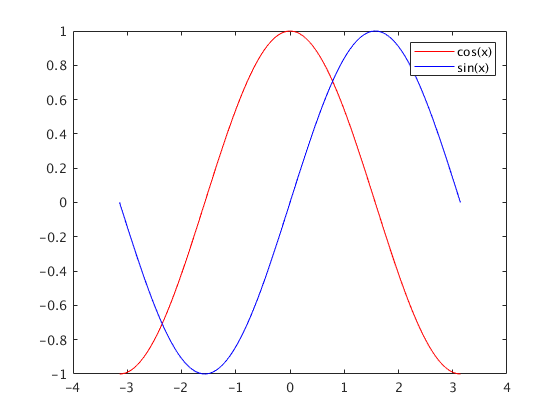
\includegraphics[width=80mm]{sin-cos-graph.png}
	\caption{Graphs of both sine and cosine}
\end{figure}

~\\
~\\
~\\
~\\
~\\

\subsection{B}

\begin{figure}[!ht]
	\centering
	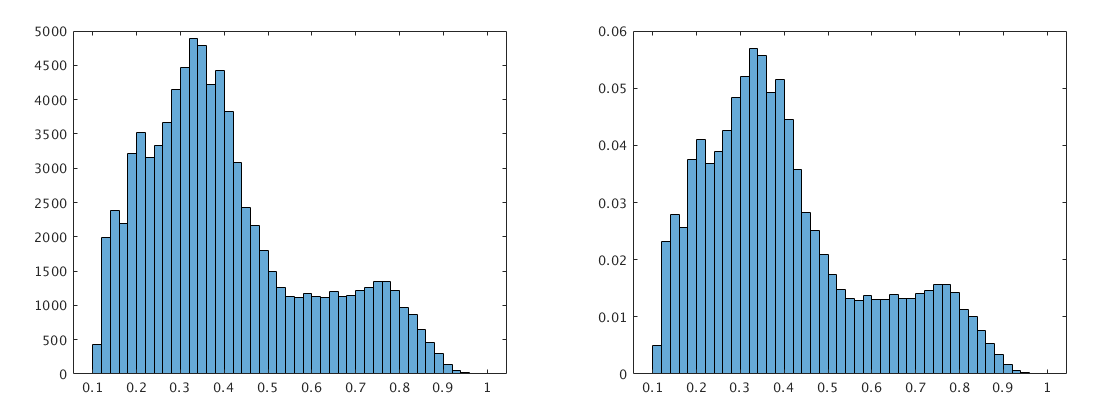
\includegraphics[width=160mm]{tiger-hist-combined.png}
	\caption{Histogram of the tiger image, normed on right (number of bins is MATLAB default)}
\end{figure}

\section{Q4}

\begin{figure}[!ht]
	\centering
	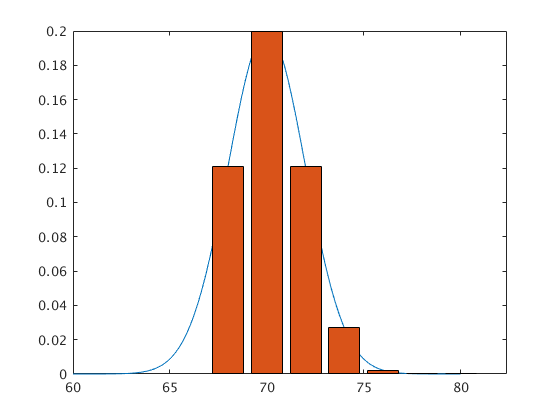
\includegraphics[width=80mm]{normal-distr-est.png}
	\caption{The normal distribution for heights adult men with bars 
		 showing an estimation method with $\delta = 2$. Note that some 
		 bars are not visible on the graph because the probabilities 
		 for them are so low.}
\end{figure}

We can also compute the sum of the bars in the nearby figure. Doing so yieds 
the result of 0.9414.

If we extend the bars in the nearby figure over a larger distance and vary the 
bar deltas, we can empirically measure how accurate such a method is, comparing 
it to one, the area under any probability density function.

As expected, lowering the bar deltas increases the accuracy substantially. Also 
expected, diminishing returns is at play here, leading to a logarithmic shape.

\begin{figure}[!ht]
	\centering
	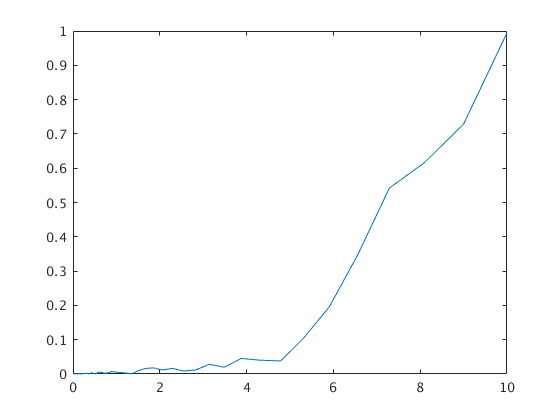
\includegraphics[width=160mm]{estimate-err.png}
	\caption{Error as a function of bar deltas}
\end{figure}

\section{Q5}

My most immediate research interest is to use both point-cloud and color video 
data to predict landslides. Though it didn't immediately strike me as a task 
that could use probabilistic graphical models, since I tend to think in terms 
of algorithms that give an exact answer, there is a lot of missing data and 
noise in real-world video and point cloud data. If I'm understanding the 
proposal that Josh linked, correctly, it sounds like most of this video data 
will be crowdsourced. In other words, that data will be from low-fidelity 
sources like cell phones. Therefore, they will not represent reality exactly. 
This is where PGMs can help. Rather than trying to find an exact answer, we can 
use probability theory to find the most \textit{likely} solution for the 
surface of the terrain geometry. While we can't reproduce the terrain geometry 
perfectly, we can certainly come up with a good estimation of it by using 
probablistic graphical models, each new video source giving a new slice of 
data, which affects the graph.

In addition to this, the task seems similar to another task that Kobus 
illustrated in his talk at the graduate meet-and-greet in April this year. The 
illustration involved generating geometry of a room from a picture of that 
room. Probablistically, I can conclude that generating geometry from cell phone 
video and point cloud data may use similar techniques.

\begin{thebibliography}{99}

\bibitem{goodfellow17}
	 Ian GoodFellow, Nicolas Papernot, Sandy Huang, Yan Duan, Pieter Abbeel, Jack Clark. 
	\textit{Attacking Machine Learning with Adversarial Examples}, 
	OpenAI Blog, 
	February 24, 2017.
    https://blog.openai.com/adversarial-example-research/

\end{thebibliography}

\end{document}